\section{Trigonometry}
\begin{align*}
\sin\theta &= \frac{Perpendicular}{Hypotenuse} & \cos\theta &= \frac{Base}{Hypotenuse} & \tan\theta &= \frac{Perpendicular}{Base} \\
\mathrm{cosec}\theta &= \frac{Hypotenuse}{Perpendicular} & \sec\theta &= \frac{Hypotenuse}{Base} & \cot\theta &= \frac{Base}{Perpendicular}
\end{align*}

From the above relations it turns out that,
\begin{align*}
\sin\theta . \mathrm{cosec}\theta &= 1 \\
\cos\theta . \sec\theta &= 1 \\
\tan\theta . \cot\theta &= 1 
\end{align*}

%---------------------------Subsection 1 ---------------- %
%-------------------------------------------------------- %
\subsection{Trigonometric Identities}
\begin{align}
%\noindent
\sin^2\theta + \cos^2\theta = 1 \\
1 + \sec^2\theta = \tan^2\theta \\
1 + \mathrm{cosec}^2\theta = \cot^2\theta
\end{align}

\begin{figure}[ht]
    \centering
    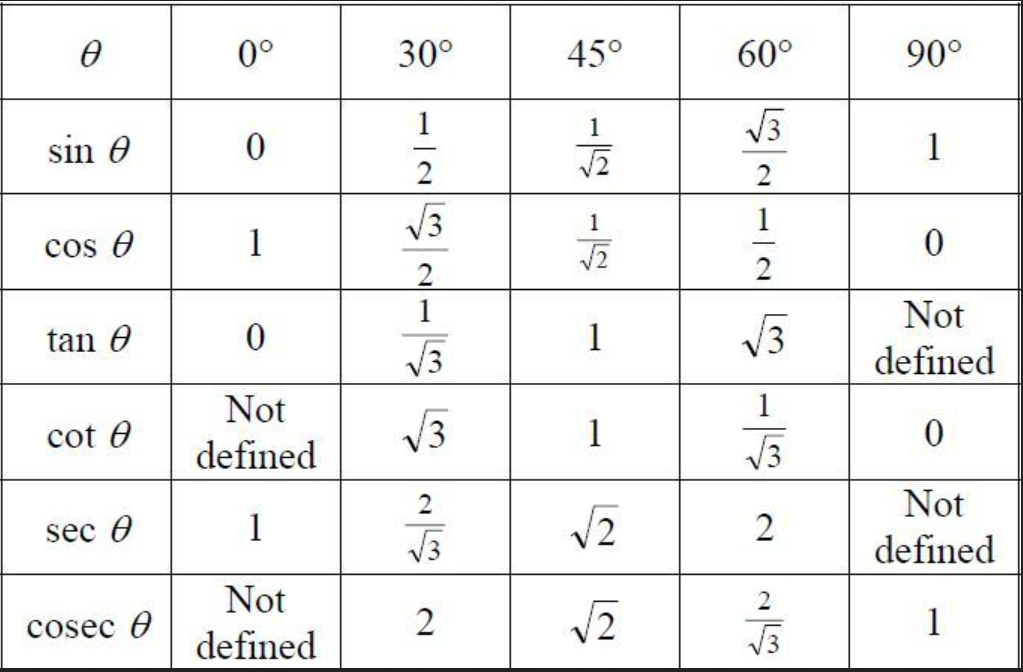
\includegraphics[scale = 0.75]{trigonometry_table}
    \caption{Most common trigonometric ratios and values}
    \label{trigonometry_values}
\end{figure}

%---------------------------Subsection 2 ---------------- %
%-------------------------------------------------------- %
\subsection{Trigonometric ratios of allied angles}
%----------------------------------------------------------
\begin{itemize}
    \item \textit{\textbf{For n being an odd multiple of $\pi/2$ the function changes to its composite function.}}
    \item \textit{\textbf{For n being an even multiple of $\pi/2$ the function does not change to its composite, but may change sign.}}
\end{itemize}

\subsubsection{First Quadrant}

%(2\pi + \theta)
\begin{align*}
\sin(2\pi + \theta) = \sin\theta \hspace{10mm} \cos(2\pi + \theta) = \cos\theta \\
\mathrm{cosec}(2\pi + \theta) = \mathrm{cosec}\theta \hspace{10mm} \sec(2\pi + \theta) = \sec\theta \\
\tan(2\pi + \theta) = \tan\theta \hspace{10mm} \cot(2\pi + \theta) = \cot\theta 
\end{align*}

%(pi\2 - \theta)
\begin{align*}
\sin(\pi/2 - \theta) = \cos\theta \hspace{10mm} \cos(\pi/2 - \theta) = \sin\theta \\
\mathrm{cosec}(\pi/2 - \theta) = \sec\theta \hspace{10mm} \sec(\pi/2 - \theta) = \mathrm{cosec}\theta \\
\tan(\pi/2 - \theta) = \cot\theta \hspace{10mm} \cot(\pi/2 - \theta) = \tan\theta 
\end{align*}
%-----------------------------------------------------------
\subsubsection{Second Quadrant}

%(pi\2 + \theta)
\begin{align*}
\sin(\pi/2 + \theta) = \cos\theta \hspace{10mm} \cos(\pi/2 + \theta) = -\sin\theta \\
\mathrm{cosec}(\pi/2 + \theta) = \sec\theta \hspace{10mm} \sec(\pi/2 + \theta) = -\mathrm{cosec}\theta \\
\tan(\pi/2 + \theta) = -\cot\theta \hspace{10mm} \cot(\pi/2 + \theta) = -\tan\theta 
\end{align*}

%(\pi - \theta)
\begin{align*}
\sin(\pi - \theta) = \sin\theta \hspace{10mm} \cos(\pi - \theta) = -\cos\theta \\
\mathrm{cosec}(\pi - \theta) = \mathrm{cosec}\theta \hspace{10mm} \sec(\pi - \theta) = -\sec\theta \\
\tan(\pi - \theta) = -\tan\theta \hspace{10mm} \cot(\pi - \theta) = -\cot\theta 
\end{align*}

%-----------------------------------------------------------
\subsubsection{Third Quadrant}

%(\pi + \theta)
\begin{align*}
\sin(\pi + \theta) = -\sin\theta \hspace{10mm} \cos(\pi + \theta) = -\cos\theta \\
\mathrm{cosec}(\pi + \theta) = \mathrm{cosec}\theta \hspace{10mm} \sec(\pi + \theta) = -\sec\theta \\
\tan(\pi + \theta) = \tan\theta \hspace{10mm} \cot(\pi + \theta) = \cot\theta 
\end{align*}

%(3pi\2 - \theta)
\begin{align*}
\sin(3\pi/2 - \theta) = -\cos\theta \hspace{10mm} \cos(3\pi/2 - \theta) = -\sin\theta \\
\mathrm{cosec}(3\pi/2 - \theta) = -\sec\theta \hspace{10mm} \sec(3\pi/2 - \theta) = -\mathrm{cosec}\theta \\
\tan(3\pi/2 - \theta) = \cot\theta \hspace{10mm} \cot(3\pi/2 - \theta) = \tan\theta 
\end{align*}

%-----------------------------------------------------------
\subsubsection{Fourth Quadrant}

%(3pi\2 + \theta)
\begin{align*}
\sin(3\pi/2 + \theta) = -\cos\theta \hspace{10mm} \cos(3\pi/2 + \theta) = \sin\theta \\
\mathrm{cosec}(3\pi/2 + \theta) = -\sec\theta \hspace{10mm} \sec(3\pi/2 + \theta) = \mathrm{cosec}\theta \\
\tan(3\pi/2 + \theta) = -\cot\theta \hspace{10mm} \cot(3\pi/2 + \theta) = -\tan\theta 
\end{align*}

%(2\pi + \theta)
\begin{align*}
\sin(2\pi - \theta) = -\sin\theta \hspace{10mm} \cos(2\pi - \theta) = \cos\theta \\
\mathrm{cosec}(2\pi - \theta) = -\mathrm{cosec}\theta \hspace{10mm} \sec(2\pi - \theta) = \sec\theta \\
\tan(2\pi - \theta) = -\tan\theta \hspace{10mm} \cot(2\pi - \theta) = -\cot\theta 
\end{align*}

%---------------------------------------------------------
\begin{itemize}
\item \textit{\textbf{The values for (2$\pi$-$\theta$) and (-$\theta$) are identical.}}
\end{itemize}

%---------------------------Subsection 3 ---------------- %
%-------------------------------------------------------- %
\subsection{Compound Angle Formulae}
\begin{align*}
\sin(A+B) &= \sin(A) \cos(B) + \cos(A) \sin(B)\\ 
\sin(A-B) &= \sin(A) \cos(B) - \cos(A) \sin(B)\\ 
\cos(A+B) &= \cos(A) \cos(B) - \sin(A) \sin(B)\\ 
\cos(A-B) &= \cos(A) \cos(B) + \sin(A) \sin(B)\\ 
\tan(A+B) &= \frac{\tan(A) + \tan(B)}{1 -\tan(A)\tan(B)}\\
\tan(A-B) &= \frac{\tan(A) - \tan(B)}{1 +\tan(A)\tan(B)} 
\end{align*}

%---------------------------Subsection 4 ---------------- %
%-------------------------------------------------------- %
\subsection{Sum or Difference Formulae}
\begin{align*}
\sin(A+B) + \sin(A-B) &=  2\sin(A)\cos(B)\\
\sin(A-B) - \sin(A-B) &=  2\cos(A)\sin(B)\\  
\cos(A+B) + \cos(A-B) &=  2\cos(A)\cos(B)\\   
\cos(A+B) - \cos(A-B) &= -2\sin(A)\sin(B)   
\end{align*}

%---------------------------Subsection 5 ---------------- %
%-------------------------------------------------------- %
\subsection{Half Angle Formulae}
\begin{align*}
\sin (\frac{A}{2}) &= \pm\sqrt{\frac{1-\cos(A)}{2}}\\
\cos (\frac{A}{2}) &= \pm\sqrt{\frac{1+\cos(A)}{2}}\\
\tan (\frac{A}{2}) &= \pm\sqrt{\frac{1-\cos(A)}{1+\cos(A)}}
\end{align*}

\vspace{-3mm} %to pull up the text

%---------------------------Subsection 6 ---------------- %
%-------------------------------------------------------- %
\subsection{Sub Multiple Angle Formulae}
\begin{align*}
\sin (2A) &= 2\sin(A)\cos(A)\\
\cos (2A) &= cos^{2}(A) - sin^{2}(A) = 2\cos^2(A) - 1 = 1 - 2\sin^2(A)\\
\tan(2A) &= \frac{2\tan(A)}{1-\tan^2(A)}\\
\sin(2A) &= \frac{2\tan(A)}{1+\tan^2(A)}\\
\cos(2A) &= \frac{1-\tan^2(A)}{1+\tan^2(A)}\\
\cos^2(A) &= \frac{1+\cos(2A)}{2}\\
\sin^2(A) &= \frac{1-\cos(2A)}{2}\\
\sin(A) &= 2\sin(A/2)\cos(A/2)\\
\cos (A) &= cos^{2}(A/2) - sin^{2}(A/2) = 2\cos^2(A/2) - 1 = 1 - 2\sin^2(A/2)
\end{align*}

%---------------------------Subsection 7 ---------------- %
%-------------------------------------------------------- %
\subsection{Triple Angle Formulae}
\begin{align*}
\sin(3x) &= 3\sin(x) - 4\sin^3(x) \\
\cos(3x) &= 4\cos^3(x) - 3\cos(x) \\
\tan(3x) &= \frac{3\tan(x) - \tan^3(x)}{1-3\tan^2(x)}\\
\sin(4x) &= 4\sin(x)\cos(x) - 8\sin^3(x)\cos(x)\\
\tan(4x) &= \frac{4\tan(x)-4\tan^3(x)}{1-6\tan^2(x)+\tan^4(x)}\\
\cos(4x) &= 8\cos^4(x) - 8\cos^2(x) + 1
\end{align*}

%---------------------------Subsection 8 ---------------- %
%-------------------------------------------------------- %

\subsection{Product Formulae}
\textit{If $A+B = C$ and $A-B = D$}\\
\textit{Then $A = (C+D)/2$ and $B = (C-D)/2$, the product formulae are defined as}

\begin{align*}
\sin(C) + \sin(D) &= 2\sin\frac{(C+D)}{2}\cos\frac{(C-D)}{2}\\
\sin(C) - \sin(D) &= 2\cos\frac{(C+D)}{2}\sin\frac{(C-D)}{2}\\
\cos(C) + \cos(D) &= 2\cos\frac{(C+D)}{2}\cos\frac{(C-D)}{2}\\
\cos(C) - \cos(D) &= -2\sin\frac{(C+D)}{2}\sin\frac{(C-D)}{2}
\end{align*}

